\section{Interface utilisateur}

Le design de ce site s'est basé sur le framework de Bootstrap qui offre un 
déploiement rapide d'un site structuré. Dans un premier temps, l'utlisateur 
fera face au portail. \\

\begin{figure}[h!]
	\centering
	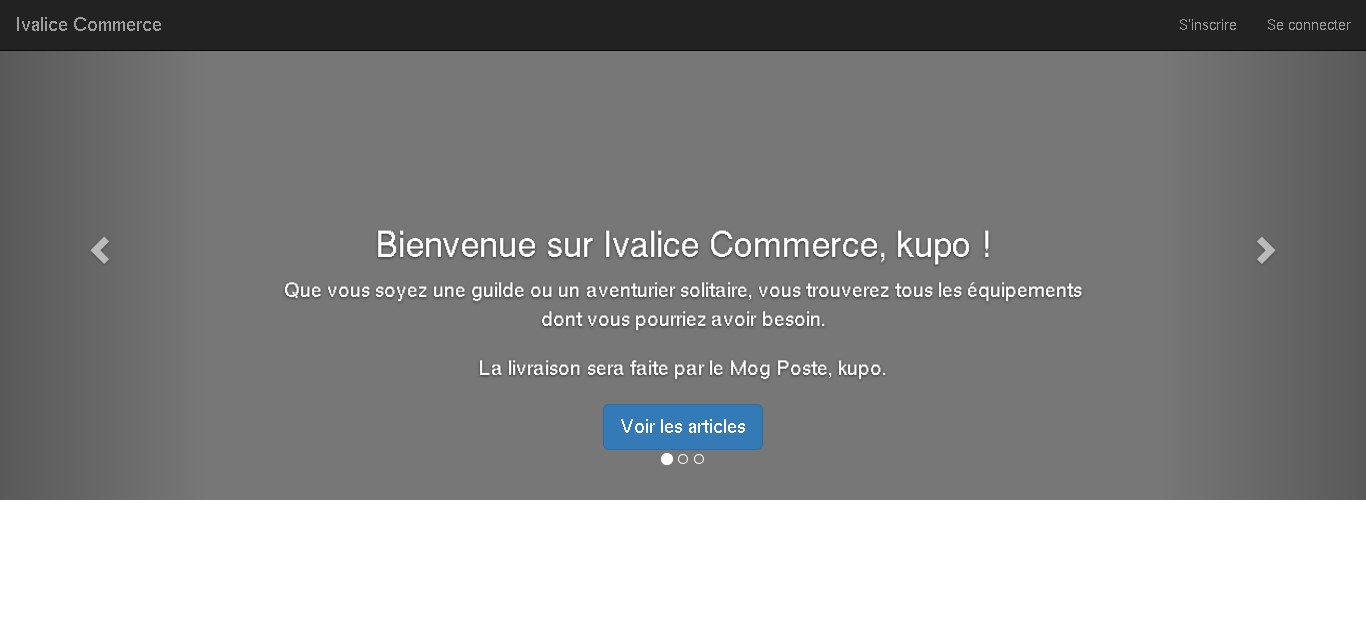
\includegraphics[width=0.8\textwidth]{img/portal.png}
	\caption{Portail}
\end{figure}

Cette page lui présente rapidement les services du site 
sur une vitrine et donne des accès rapides à d'autres pages (une liste de produits pour les 
non membres, un lien vers la page d'inscription ou de connexion). \\

\begin{figure}[h!]
	\centering
	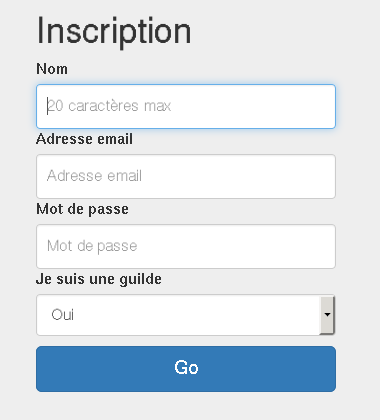
\includegraphics[width=0.3\textwidth]{img/signup.png}
	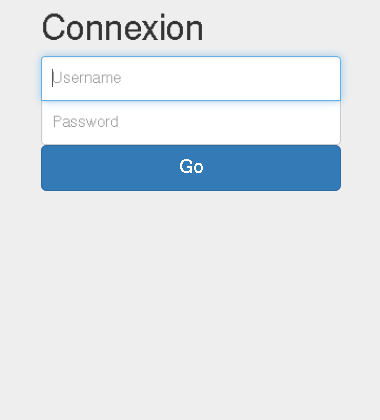
\includegraphics[width=0.3\textwidth]{img/login.png}
	\caption{Formulaire d'inscription et de connexion}
\end{figure}

Une fois connecté, on arrive à une page d'index qui affiche la liste des produits. 
Il y a un menu latéral qui lui permet de filtrer la liste des produits. Dans le 
tableau récapitulant les produits, il se trouve des boutons d'action qui 
permettent d'ajouter ou de retirer une unité de ce produit dans le panier. \\

\begin{figure}[h!]
	\centering
	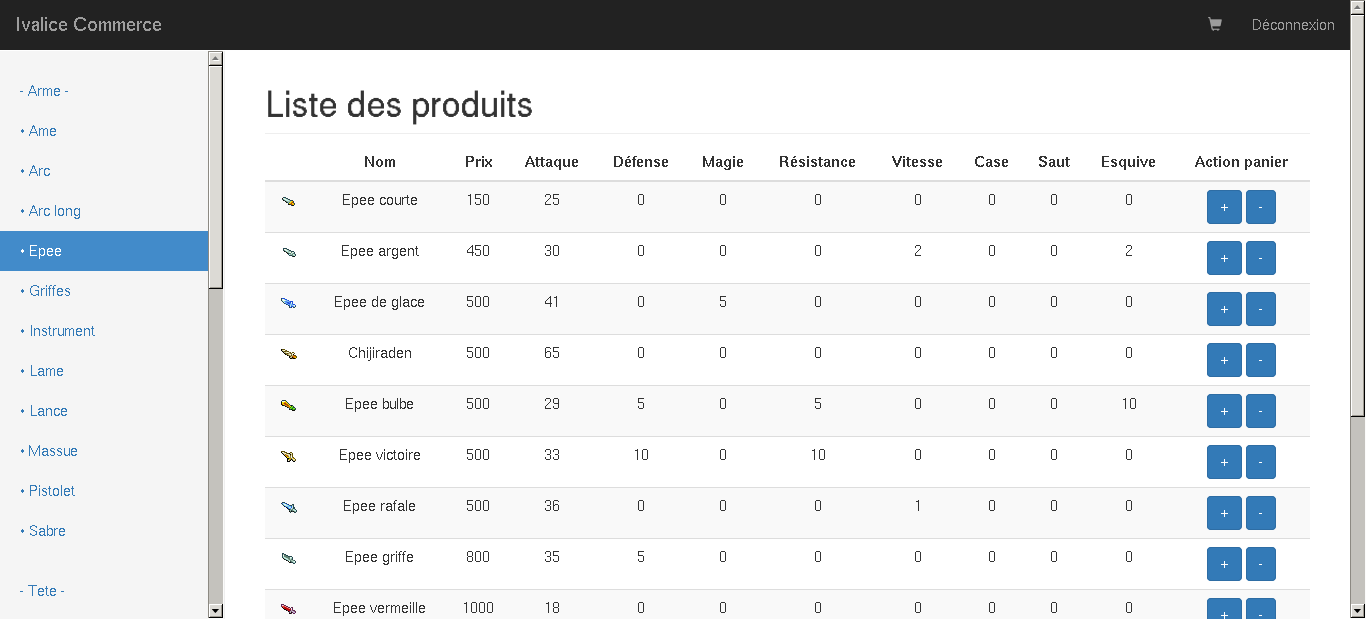
\includegraphics[width=0.8\textwidth]{img/index.png}
	\caption{Liste des produits filtrée (Epée)}
\end{figure}

\newpage
Sur la page du panier, les produits sélectionnés par l'utilisateur sont listés 
et le prix total est indiqué. Si le membre est une guilde, le total serait 
indiqué en rouge avec une réudction de 5\%. Il lui est aussi possible de 
retirer des produits directement à partir du panier. \\

\begin{figure}[h!]
	\centering
	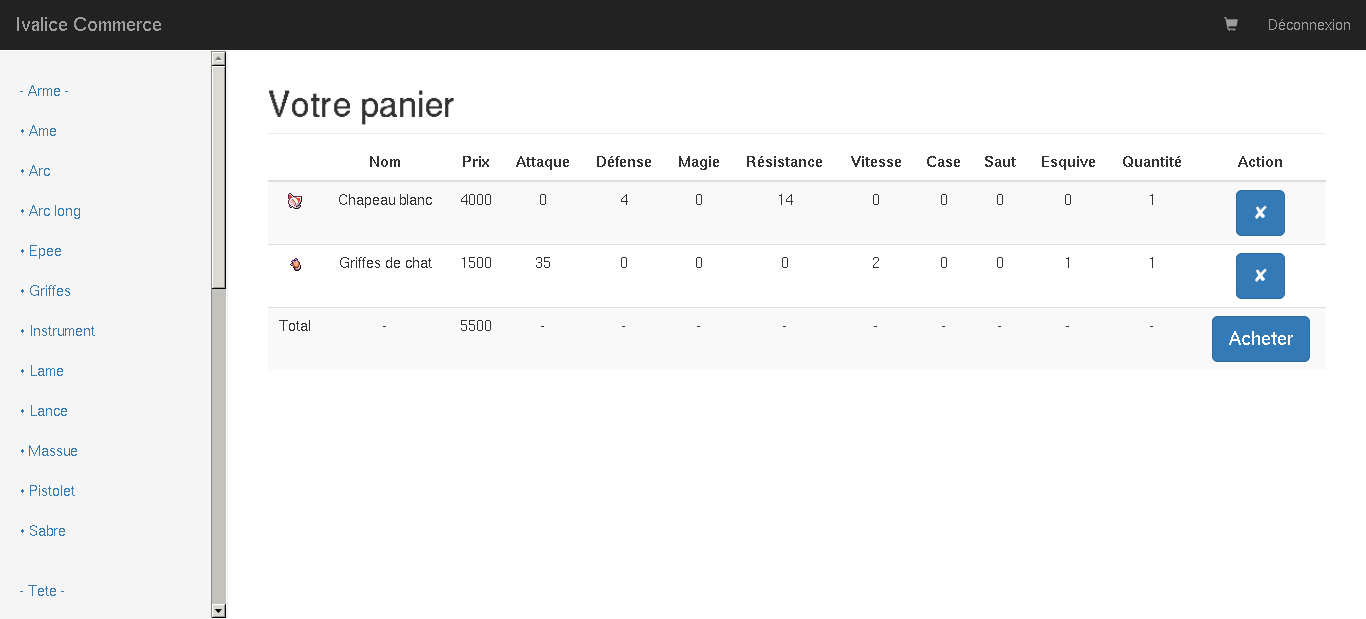
\includegraphics[width=0.8\textwidth]{img/cart.png}
	\caption{Panier d'un membre non guilde}
\end{figure}

Il ne reste donc plus qu'à acheter l'ensemble des produits dans le panier. On 
arrive sur une page confirmant que l'achat a été effectué. Le panier de 
l'utilisateur est donc vidé à l'occasion. \\

\begin{figure}[h!]
	\centering
	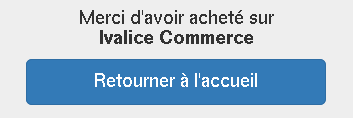
\includegraphics[width=0.6\textwidth]{img/buy.png}
	\caption{Confirmation d'achat}
\end{figure}

Enfin, si un utilisateur essaie de s'inscrire avec des identifiants déjà 
existants, ou s'il se connecte avec des mauvais identifiants, il sera renvoyé au 
portail avec des messages d'erreur. \\

\begin{figure}[h!]
	\centering
	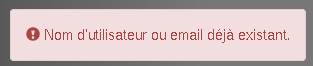
\includegraphics{img/trysignup.png}
	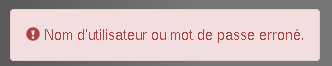
\includegraphics{img/trylogin.png}
	\caption{Messages d'erreur pour inscription ou connexion échouée}
\end{figure}

